\documentclass{standalone}
\usepackage{amsmath, amsthm, amssymb, amsbsy}
\usepackage{textgreek, upgreek, gensymb, mathtools, extarrows}
\usepackage{tikz}
\usetikzlibrary{patterns,matrix,positioning,shapes}
\begin{document}
  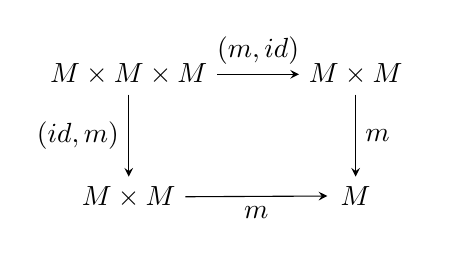
\begin{tikzpicture}
    \matrix (m) [matrix of math nodes,
                 row sep=3em, column sep=3em, minimum width=2em]{
       M \times M \times M & M \times M \\
       M \times M          & M \\};
    \path[-stealth]
      (m-1-1) edge node [above] {$(m, id)$} (m-1-2)
      (m-1-1) edge node [left] {$(id, m)$} (m-2-1)
      (m-1-2) edge node [right] {$m$} (m-2-2)
      (m-2-1) edge node [below] {$m$} (m-2-2);
  \end{tikzpicture}
\end{document}
